\chapter{Methods}

\section{Sampling Images}

It is not feasible for every image in the NTCIR-12 LSAT data set to be annotated manually. The collection is very large, containing 88,125 images. Moreover it is even more unfeasible to annotate every image four times (for each annotation methodology), thus sampling images to reduce the number of images to annotate is necessary. There are two methodologies employed to sample images: The first builds upon previous work~\cite{scells2016qut} which identifies a way of clustering lifelog images using image histograms for features; and aligning the images temporally to determine cluster segmentation boundaries\footnote{\url{https://github.com/hscells/lifelog-sampling}}. After clustering images, the sampling technique involves selecting one image at random from each cluster. The cosine similarity measure is used to determine if an image should be added to an existing cluster. The threshold value of the cosine between two images is set to 0.86\footnote{This value was empirically found to provide a range of sufficiently different clusters, each containing similar images}. Clusters are then combined based on visual similarity using the aforementioned image histograms and a representative image from each of these clusters is chosen at random. This process results in about 16,000 images for annotation. The second sampling method entails processing the qrels to extract only the relevant images. A maximum of 30 images are selected from each of the 48 topics which results in just over 1,000 images required for annotation. Some topics have less than 30 relevant images which is why the total number of images is lower than what one would expect.

There is some overlap between the images chosen from the clustering process and the images that are known to be relevant, however it overall reduces the number of images to annotate by around 80\%. In reality, it is not expected that all of these images are annotated, rather, the smaller sample set should provide a reasonable interpolation of the larger data set. Annotating both relevant and non-relevant images ensures that retrieval is working correctly: both relevant and non-relevant images should be retrieved, however the images annotated with relevant annotations should rank higher.

The sampled images are uploaded to a database to be annotated. Annotations are then collected through specially designed interfaces.
% Both sampling techniques are required 
% For future work, a combination of clustering and matching images to relevant topics might be a better option, as there will most likely be many irrelevant annotations. There may also be no annotations which are relevant to a topic as well, since the sampling is somewhat random. This makes the process less than idea, but will serve as a proof of concept for further research.

\section{Collecting Annotations}

Once the images have been sampled and uploaded into a database, they are ready to be annotated. Four web interfaces are used to collect of annotations\footnote{\url{https://github.com/hscells/lifelog-ia}}. The interfaces allow experts to annotate images selected randomly from a list of unannotated images. It is important to note that each image is annotated only once and an attempt is made to ensure that there is an overlap between the images and the annotations such that most images annotated should have four annotations.

The architecture of the interfaces consists of:
\begin{enumerate}
    \item A database to store the annotations and the sampled images. The database also records statistical data about each user performing the annotations: who annotated each image, and how long it takes to perform an annotation. This ensures there is a record of who annotated each image, and allows a statistical analysis to be performed at a later stage.
    \item A web server and that handles the `business logic'. This server exposes some password protected RESTful services that applications can hook into.
    \item A website which consumes the API provided by the web server and handles `view logic'. This is the layer that annotators interact with directly. Each interface is one of these views.
\end{enumerate}

The interfaces are designed with great care to ensure collecting annotations is as painless as possible. It is important that the total time it takes to annotate an image (including the time between annotating images, i.e. loading an image) is as small as possible; If it takes a minute to annotate one image, it will take an hour to annotate only 60 images.

% It is for this reason that an automatic captioning system is used to caption the rest of the images. For each methodology, annotations will be generated using a state-of-the-art machine learning architecture. This ensures every single image is annotated, so an annotation has been collected for each image, for each annotation methodology.

\section{Annotation Methodologies}

Four annotation methodologies are selected for investigation: \textbf{textual}, \textbf{tags}, \textbf{relevance assessment} and \textbf{reverse query}. While the annotation types are wildly different to each other, they are all collected in a very similar way. An expert annotator is shown a randomly chosen image from the sampled set of images and is asked to provide an annotation (or in the case of relevance assessment, multiple annotations) for the image. The interfaces used for collecting annotations are pictured and described as follows:

\textbf{Textual}

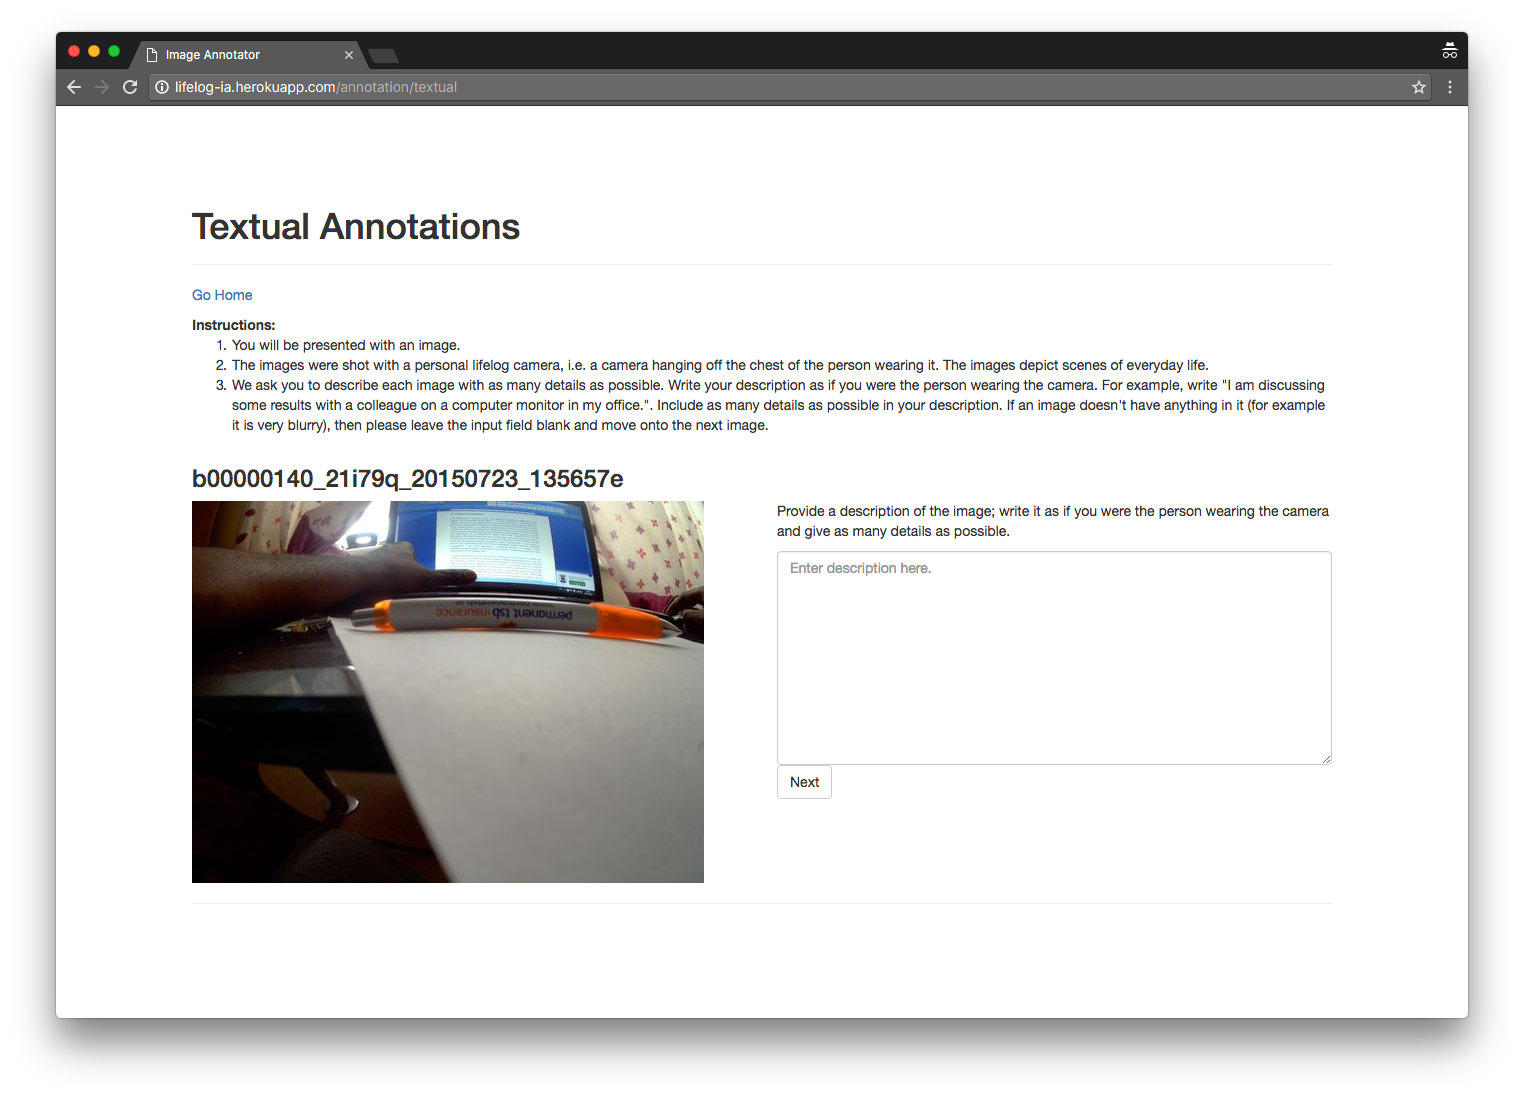
\includegraphics[width=0.95\textwidth]{images/text-interface}

Here, annotations are collected using free form text through a text box on the page. Each textual annotation should contain semantic information about an image, and describe the image with as much detail as possible. These annotations are very similar to a textual document in a typical web search engine, which is why they are selected as one of the methodologies to investigate. Information retrieval is commonly associated with textual documents which contain many sentences with varied semantic and contextual information. This type of annotation highly resembles typical document retrieval and can almost be seen as a baseline, whereas the other annotation methodologies are somewhat novel.

\newpage
\textbf{Tags}

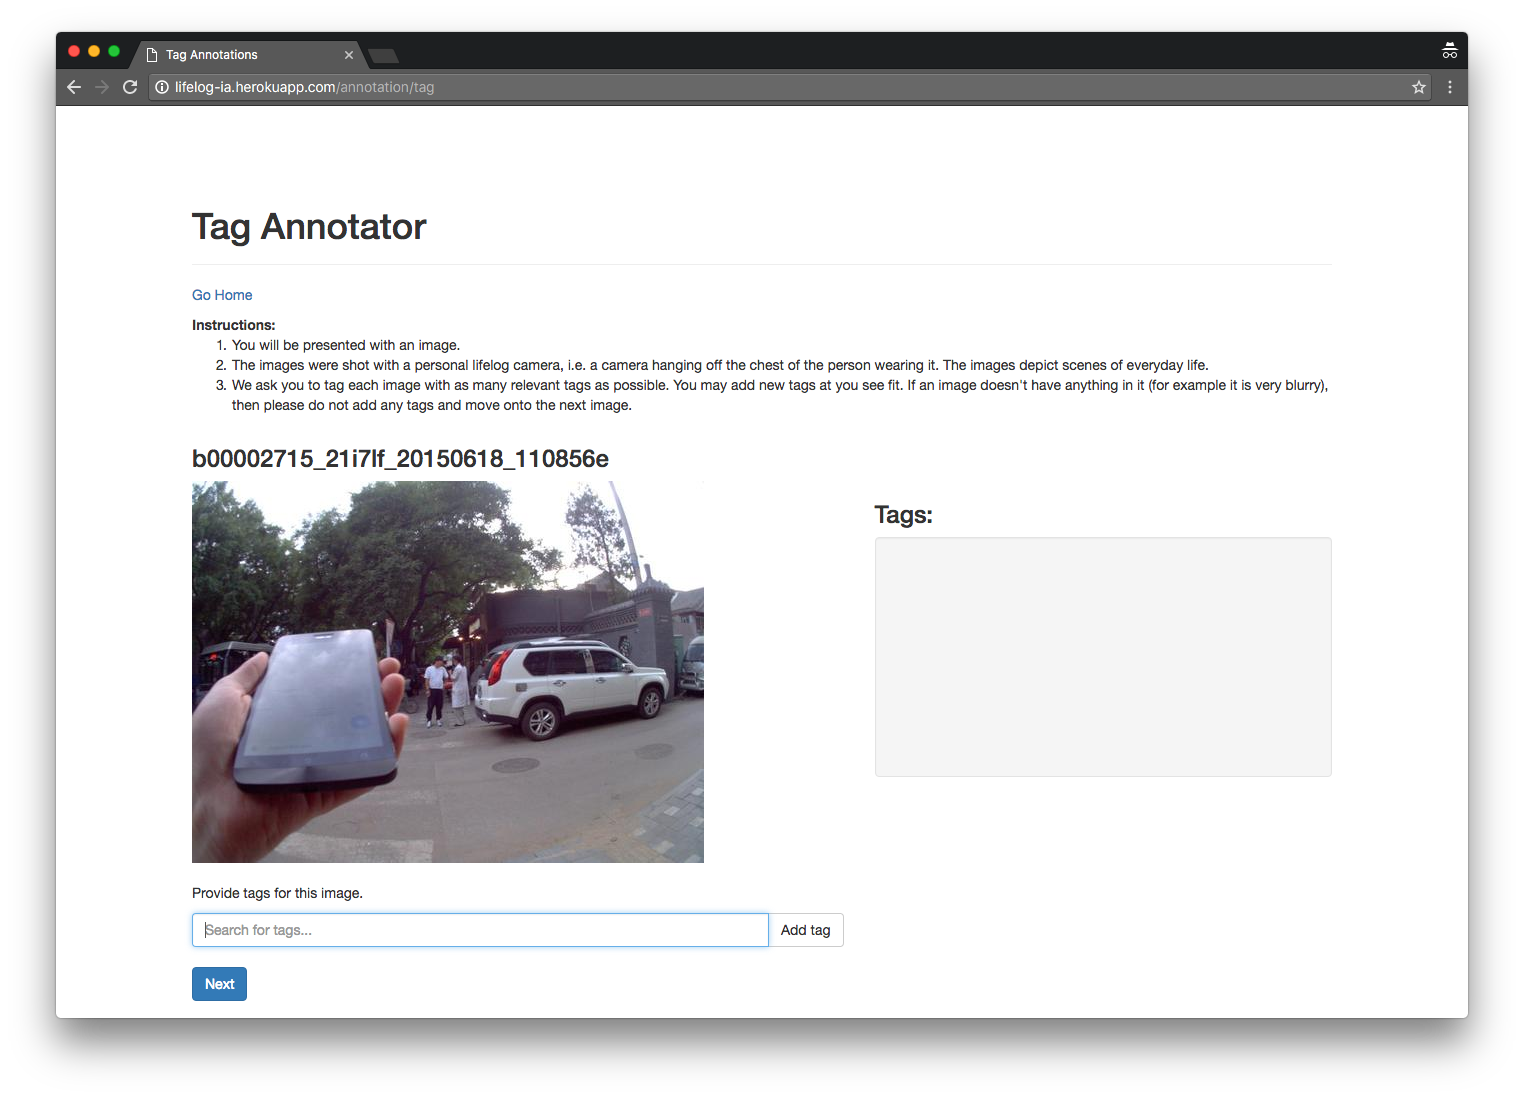
\includegraphics[width=0.95\textwidth]{images/tag-interface}

Tags are collected through this specifically designed interface. The vocabulary of tags is created from previously added tags, the list of tags available is arbitrary and can be expanded. This annotation methodology and style of collection is similar to that seen in other online image tagging scenarios such as Flickr. Similarly, the vocabulary is not restricted to a preset group of terms. This unrestricted vocabulary can result in human error (spelling mistakes), but allows for precise observations about key objects or events in an image. The tags that annotators are allowed to input are allowed to contain more than one word, to cover concepts like `train station' or `shopping mall'.

\newpage
\textbf{Reverse Query}

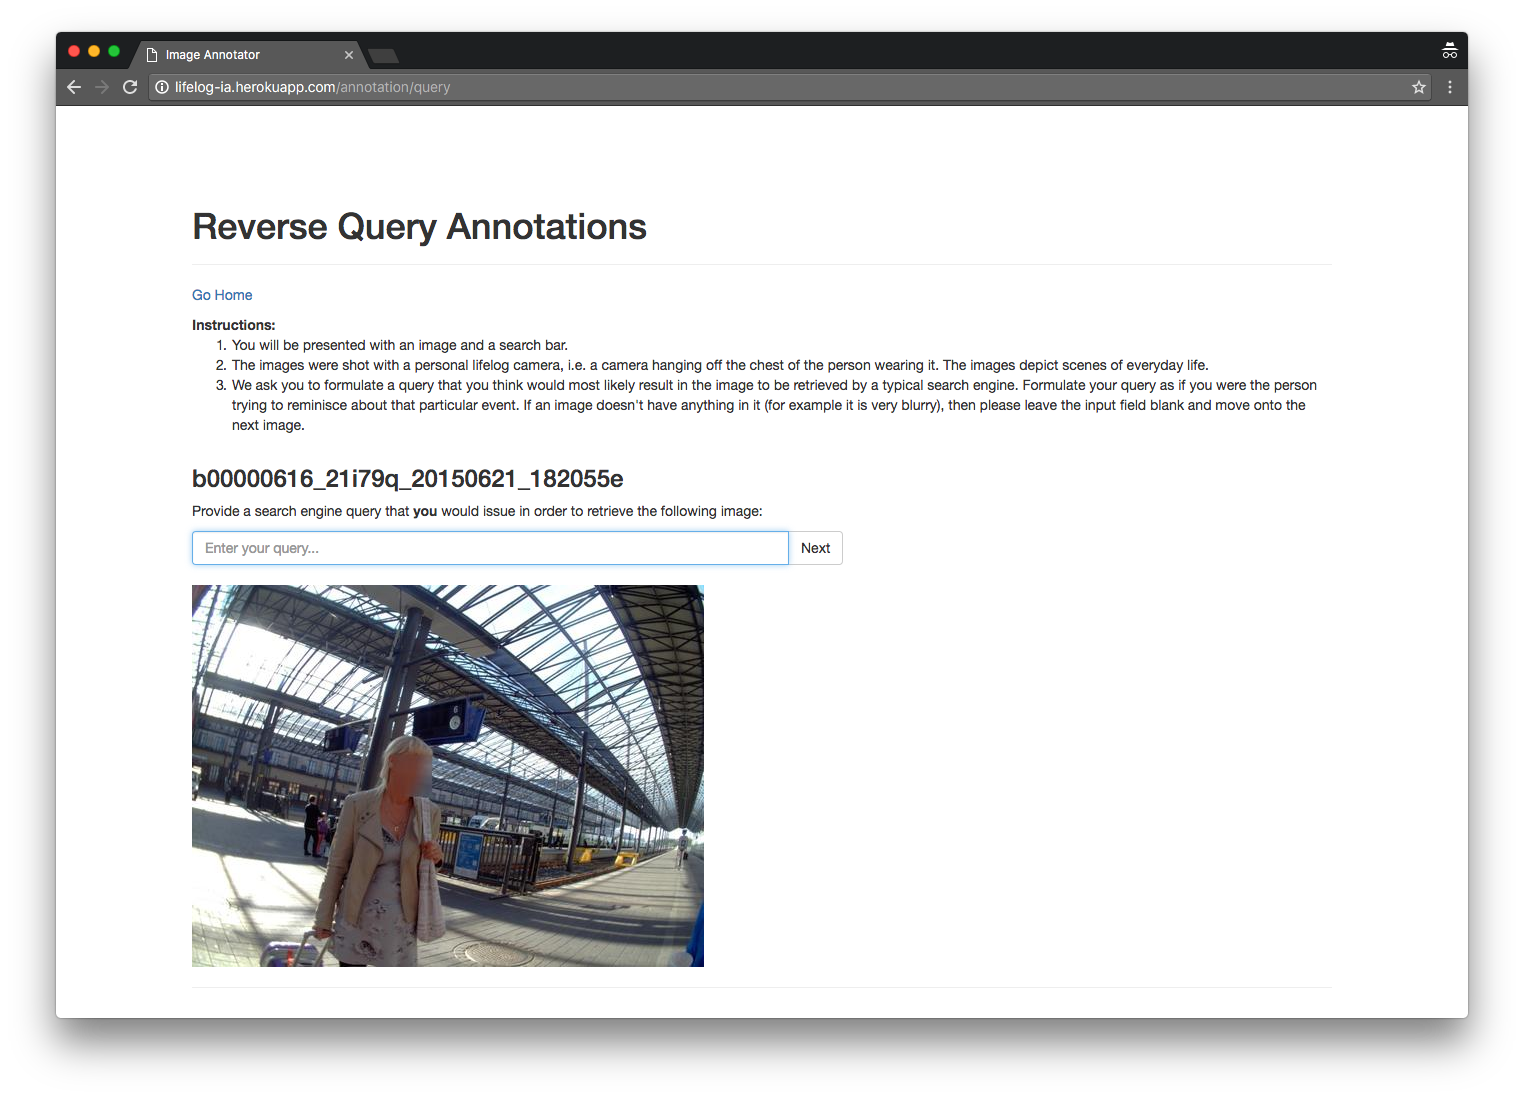
\includegraphics[width=0.95\textwidth]{images/query-interface}

In this interface, user queries are collected by presenting an image taken from the lifelog camera and asking the annotator to provide a query with what they expect to be returned by a typical search engine. This is a relatively novel way of annotating \textit{any} type of document or image~\cite{quteprints82599}. This form of annotation represents the query logs from a search engine. Search engine companies have this data but generally do not make this available due to privacy concerns~\cite{silvestri2010mining}. These annotations are less focused on detail and more focused on one to two key objects or events in the image.

\newpage
\textbf{Relevance Assessment}

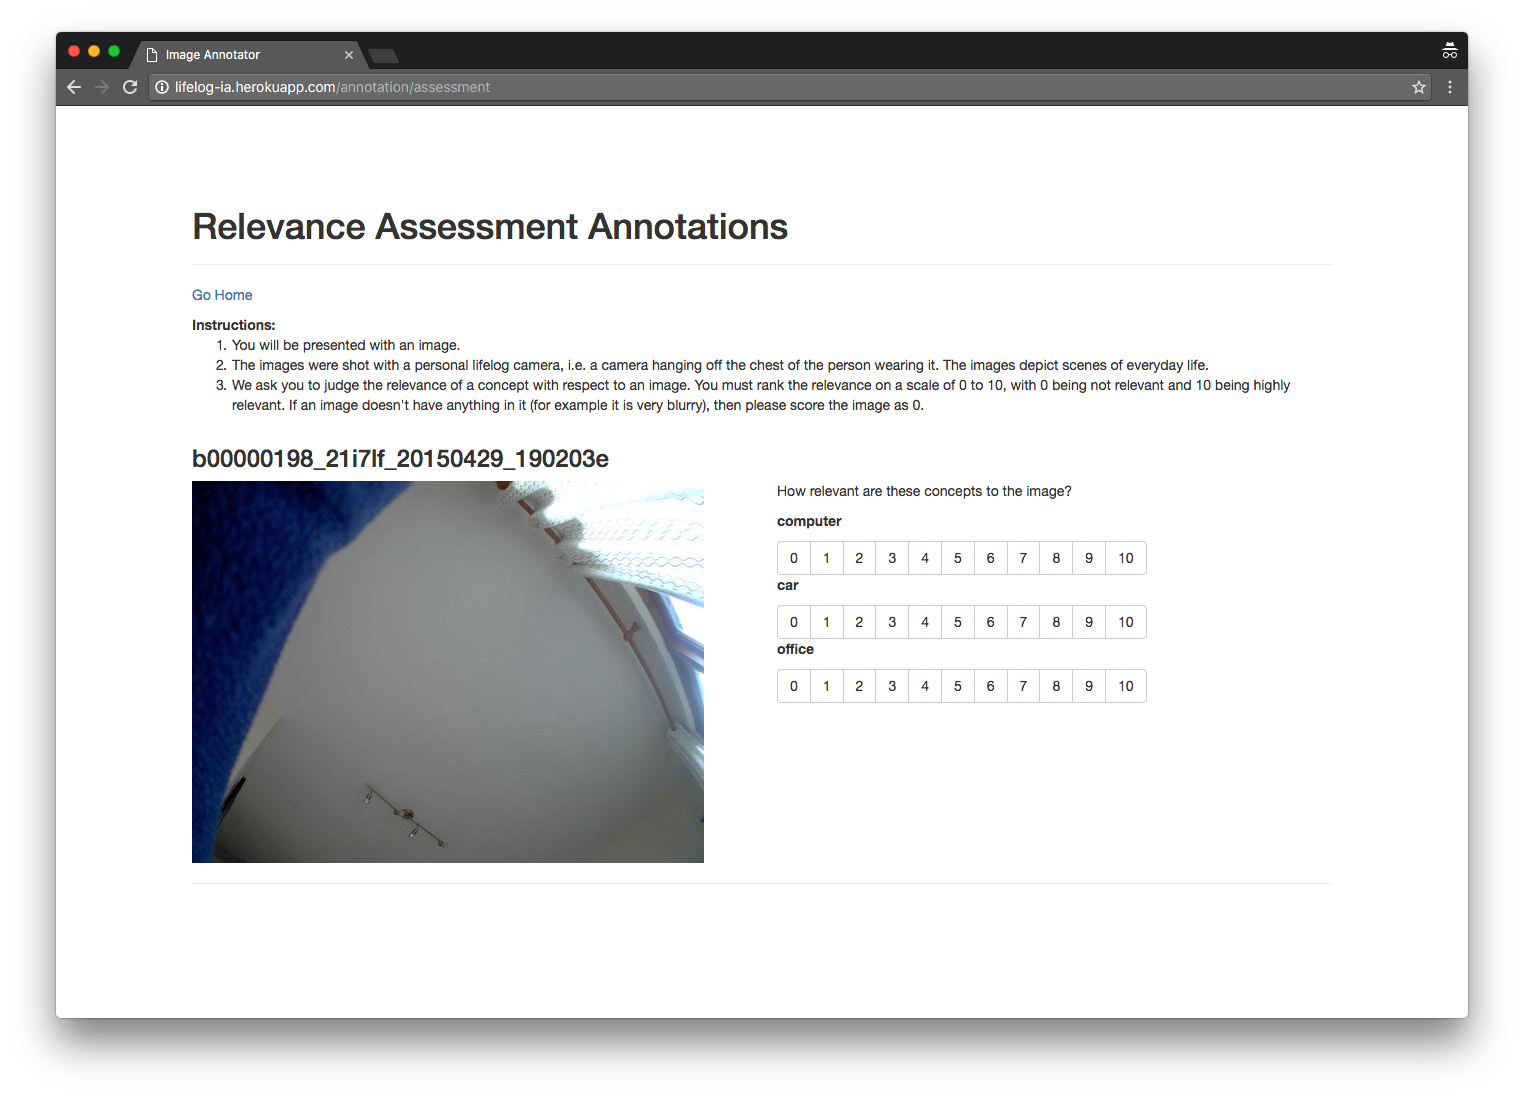
\includegraphics[width=0.95\textwidth]{images/rel-ass-interface}

Relevance assessment involves presenting an annotator with an image, and asking them to judge how relevant a concept is to the image. Assessors are asked to choose concepts from a list to assess, and from those chosen concepts are asked to assess the relevance of that concept to the target image. Concepts are ranked on a scale of zero to ten, where zero is not relevant at all and ten is highly relevant.

These annotations are similar to the tag annotations in that annotators are annotating with some notion of a `concept'. The major difference between the two annotation methodologies is that the vocabulary is finite and the relevance of a concept to the target image is not binary.

Relevance assessment annotations are collected last, the list of concepts is formed from analysing terms in the other annotations. Concepts are chosen by creating a list of terms from the existing textual, tag and query annotations, which are then filtered to the terms that occur in the NTCIR-12 LSAT topic titles and descriptions. Each term is scored using IDF\footnote{Inverse Document Frequency} and then ranked using an algorithm similar to discounted cumulative gain~\cite{jarvelin2002cumulated}; in which higher scoring terms are selected less frequently, and more emphasis is placed on selecting lower scoring terms. 

\newpage
\textbf{Automatic Image Annotation}

Finally, an attempt to automatically caption images for each annotation methodology is done by utilising a recent state-of-the-art machine learning image captioning approach~\cite{karpathy2015deep} which has been open sourced\footnote{\url{https://github.com/karpathy/neuraltalk2}}. The architecture of the system consists of the final hidden layer of a convolutional neural network (CNN) which learns features of image regions being fed into a recurrent neural network (RNN) that generates textual descriptions.

A model is trained in the system described above using the $adam$ optimiser with $\alpha$ set to 0.8 and $\beta$ set to 0.999. The learning rate of the language model is set to 0.0004. Two training attempts are performed: one where the model is trained for a maximum of 70,000 iterations, and another where the model is trained for a maximum of 300,000 iterations. More iterations are performed afterwards to fine tune the deep learning architecture, but in all cases the changes to values of the optimisation function are insignificant.

\section{Evaluating Annotations}\label{methods:evaluating}

Annotations are evaluated with an ad-hoc, TREC style methodology. The topics and qrels from the NTCIR-12 Lifelog semantic access pilot task are used to perform evaluation. In total eight runs are produced: five consisting of each of the manually annotated annotations plus the combination of these, and another four consisting of automatically generated captions for textual, tag, and query annotations as well as the combination of these. This is to investigate if any correlations betweent the manually annotated annotations and the automatic annotations exist, and to determine if an automatic system can effectively generate suitable annotations for lifelog images. It should be noted that the relevance assessment annotations cannot be learnt by the neural network framework used simply due to the format of the annotatinons.

Document rankings are generated by submitting queries to ElasticSearch using porter stemmer and a default English stoplist. Queries are formulated by using the title field from the NTCIR-12 Lifelog topics. The stemming and stopping are also applied to the queries. ElasticSearch is also set to only retrieve a maximum of 1,000 images. The runs produced by this system are evaluated using \verb|trec_eval| and the NTCIR-12 Lifelog qrels. The retrieval model for producing runs is $tf*idf$ and the method is the default \verb|simple query string|\footnote{\url{https://www.elastic.co/guide/en/elasticsearch/reference/current/query-dsl-query-string-query.html}} query.

The document rankings and evaluation is performed through a custom-built framework\footnote{\url{https://github.com/hscells/lifelog-eval}}. A Java RESTful application wraps Elasticsearch. This is so a query issued to the Java application can return a properly formatted TREC run, and so many queries can be issued with one request. Rather than the system producing a search listing, it outputs in a format ready for \verb|trec_eval| to process.
